\documentclass[12pt]{article}

%***************************************************************************************************
% Math
\usepackage{fancyhdr} 
\usepackage{amsfonts}
\usepackage{amsmath}
\usepackage{amssymb}
\usepackage{amsthm}
%\usepackage{dsfont}

%***************************************************************************************************
% Macros
\usepackage{calc}

%***************************************************************************************************
% Commands and Custom Variables	
\newcommand{\problem}[1]{\hspace{-4 ex} \large \textbf{Problem #1} }
\let\oldemptyset\emptyset
\let\emptyset\varnothing
\newcommand{\norm}[1]{\left\lVert#1\right\rVert}
\newcommand{\sint}{\text{s}\kern-5pt\int}
\newcommand{\powerset}{\mathcal{P}}
\renewenvironment{proof}{\hspace{-4 ex} \emph{Proof}:}{\qed}

%***************************************************************************************************
%page
\usepackage[margin=1in]{geometry}
\usepackage{setspace}
%\doublespacing
\allowdisplaybreaks
\pagestyle{fancy}
\fancyhf{}
\rhead{Shaw \space \thepage}
\setlength\parindent{0pt}

%***************************************************************************************************
%Code
\usepackage{listings}
\usepackage{courier}
\lstset{
	language=Python,
	showstringspaces=false,
	formfeed=newpage,
	tabsize=4,
	commentstyle=\itshape,
	basicstyle=\ttfamily,
}

%***************************************************************************************************
%Images
\usepackage{graphicx}
\graphicspath{ {images/} }
\usepackage{float}

%tikz
\usepackage[utf8]{inputenc}
\usepackage{pgfplots}
\usepgfplotslibrary{groupplots}

%***************************************************************************************************
%Hyperlinks
%\usepackage{hyperref}
%\hypersetup{
%	colorlinks=true,
%	linkcolor=blue,
%	filecolor=magenta,      
%	urlcolor=cyan,
%}


\begin{document}
	\thispagestyle{empty}
	
	\begin{flushright}
		Sage Shaw \\
		m565 - Fall 2017 \\
		\today
	\end{flushright}
	
{\large \textbf{HW 4}}\bigbreak

%***************************************************************************************************
\singlespacing
\problem{1} We write Lagrange's interpolation formula as 
$$ \sum\limits_{j=0}^n l_j(x)f(x_j)  $$
Show that 
\begin{align}
	\sum\limits_{j=0}^n l_j(x)x_j \equiv x
\end{align}
	
	\doublespacing
	\begin{proof}
		Consider the function $f(x)=x$. Given the sample points $\{x_j\}_{0=j}^n$, $f(x_j)=x_j$. Since $f$ is a polynomial, it is the polynomial that interpolates the points $\Big \{ \big(x_j,f(x_j) \big) \Big\}_{0=j}^n$ and thus
		$$ \sum\limits_{j=0}^n l_j(x)x_j = \sum\limits_{j=0}^n l_j(x)f(x_j) = f(x) = x$$
	\end{proof}


%***************************************************************************************************
\singlespacing
\problem{2} Let $$E_1(x) = \int_{x}^{\infty}\frac{e^{-t}}{t}dt \ \ x>0$$ 
We would like to construct a table of values over the interval $x \in [1,10]$ such that the second degree polynomial interpolation between any three adjacent points in the table will give an error less than or equal to $10^{-8}$.

	We will use the error formula
	$$
	\vert P_2(x) - f(x) \vert \leq \frac{\vert (x-x_0)(x-x_1)(x-x_2) \vert}{3!} \max_{a\leq x \leq b} \big\vert f^{(3)}(x) \big\vert
	$$
	First we will find the maximum of the third derivative over $1 \leq x \leq 10$.
	\begin{align*}
		f^{\prime}(x) & = \frac{d}{dx} \int_{x}^{\infty}\frac{e^{-t}}{t}dt \\
		& = \frac{d}{dx} -\int_{\infty}^{x}\frac{e^{-t}}{t}dt \\
		& = -\frac{e^{-x}}{x} \\
		& = -x^{-1}e^{-x} \\
		f^{\prime\prime}(x) & = \frac{d}{dx} -x^{-1}e^{-x} \\
		& = x^{-2} e^{-x} + x^{-1}e^{-x} \\
		f^{(3)}(x) & = \frac{d}{dx} (x^{-2} e^{-x} + x^{-1}e^{-x}) \\
		& = -2x^{-3}e^{-x} - x^{-2} e^{-x} - x^{-2} e^{-x} - x^{-1}e^{-x} \\
		& = -2x^{-3}e^{-x} - 2x^{-2} e^{-x} - x^{-1}e^{-x} \\
		& = (-2x^{-3} - 2x^{-2} - x^{-1}) e^{-x}
	\end{align*}
	This function has no local extrema except at the end points. It is clear that the maximum value of the absolute value of the third derivative is at $x=1$, thus $\max_{1\leq x \leq 10} \big\vert f^{(3)}(x) \big\vert = \tfrac{5}{e}$. \bigbreak
	
	Next we will find the maximum value of $\vert (x-x_0)(x-x_1)(x-x_2) \vert$ over our interval. Note that if $x$ is one of our data points, this product is zero. Without loss of generality we can assume that $x_0 < x < x_1$ for some ordered points $x_0 < x_1 < x_2$. Since all of our points are equally spaced, $\vert x_0 - x_1 \vert = \vert x_1 - x_2 \vert = h$ where $h$ is the step size in our table. Letting $ x-x_0 = w$ we have the following substitutions $ x_1-x = h-w, x_2 - x = 2h - w$. Now our problem is to find the maximum value of $ w(w-h)(w-2h)$ for $ 0 \leq w \leq h$. Note that each term is positive so we may drop the absolute. Distributing we have $w^3 - 3w^2h + 2wh^2$. To maximize this we find the root of the derivative $3w^2 + 6wh + 2h^2$. Applying the quadratic formula we find that our function has a maximum at 
	$$
	w = \frac{-6h \pm \sqrt{(6h)^2 - 4(3)(2h^2)}}{2(3)} = h \frac{3-\sqrt{3}}{3}
	$$
	Substituting this back in we have the maximum value
	$$
	(h \tfrac{3-\sqrt{3}}{3})^3 - 3(h \tfrac{3-\sqrt{3}}{3})^2h + 2(h \tfrac{3-\sqrt{3}}{3})h^2 = \frac{2 \sqrt{3}}{9}h^3
	$$
	Finally we get that our error is bounded by
	$$
	\vert P_2(x) - f(x) \vert \leq \frac{5\sqrt{3}}{27e}h^3
	$$
	If we would like our error to be below $10^{-8}$ we simplify $\frac{5\sqrt{3}}{27e}h^3 < 10^{-8}$ to obtain a maximum step size
	$$
	h < \sqrt[3]{\frac{27e10^{-8}}{5 \sqrt{3}}} \approx 0.00439
	$$
	
%***************************************************************************************************
\singlespacing
\problem{3}

%***************************************************************************************************
\problem{4 (a)} Create a program for interpolating data using the the barycentric formula.

	\begin{lstlisting}
def polyinterp(u, x, y, w=None):
	if w == None:
		w = baryweights(x)
	ret = np.zeros(len(u))
	for i in range(len(ret)):
		if u[i] in x:
			ret[i] = y[np.where(x==u[i])]
		else:
			weights = w /(u[i] - x)
			ret[i] = weights.dot(y)/sum(weights)
	return ret

def baryweights(x):
	w = np.ones(len(x))
	for j, xj in enumerate(x):
		for xi in x[np.arange(len(x))!=j]: 
			w[j] /= (xj - xi)
	return w
	\end{lstlisting}

%***************************************************************************************************
\problem{4 (b)} Using equispaced points, the Chebyshev points of the first and second kind, and Legendre points, interpolate $f(x) = \sqrt{x^2 +.1}$ using 15 points. Evaluate it at 201 equally spaced points on the interval $[-1,1]$, and plot the error. Decide which point set produces the best result?

	\begin{lstlisting}
def p4b():
	samples = []
	labels = []
	x = np.linspace(-1,1,15)
	samples.append(x)
	labels.append('Equispaced points:')
	x = []
	for j in range(0,15):
		x.append( -1* np.cos( (2*j+1)/29 * np.pi))
	samples.append(np.array(x))
	labels.append('First kind Chebyshev points:')
	x = []
	for j in range(0,15):
		x.append( -1* np.cos( (j*np.pi)/14 ) )
	samples.append(np.array(x))
	labels.append('Second kind Chebyshev points:')
	x = [-0.987992518020485,
			-0.394151347077563,
			0.570972172608539,
			-0.937273392400706,
			-0.201194093997435,
			0.724417731360170,
			-0.848206583410427,
			0,
			0.848206583410427,
			-0.724417731360170,
			0.201194093997435,
			0.937273392400706,
			-0.570972172608539,
			0.394151347077563,
			0.987992518020485]
	samples.append(np.array(x))
	labels.append('Legendre points:')
	for x, l in zip(samples, labels):
		y = p4_foo(x)
		u = np.linspace(-1,1,201)
		p = polyinterp(u, x, y)
		f = p4_foo(u)
		print(l)
		print('Eucidian norm: %f' % np.linalg.norm(f-p))
		print('Infinity norm: %f' % np.linalg.norm(f-p,np.inf))
		plt.subplot(2,1,1)
		plt.plot(u,p, 'r-')
		plt.plot(u,f, 'k-')
		plt.plot(x,y, 'bo')
		plt.xlim( (-1, 1) )
		plt.ylim( (.2, 1.2) )
		
		plt.subplot(2,1,2)
		plt.plot(u, p-f, 'k-')
		plt.xlim( (-1, 1) )
		y_range = np.max( np.abs(p-f) )
		plt.ylim( (-y_range, y_range) )
		plt.show()
	\end{lstlisting}
	
	The code above gives the following output.
	\begin{lstlisting}
Equispaced points
Eucidian norm: 0.084877
Infinity norm: 0.024440
First kind Chebyshev points
Eucidian norm: 0.001745
Infinity norm: 0.000205
Second kind Chebyshev points
Eucidian norm: 0.001945
Infinity norm: 0.000266
Legendre points
Eucidian norm: 0.001945
Infinity norm: 0.000621
	\end{lstlisting}
	
	\begin{figure}[H]
		\caption{Equispaced points}
		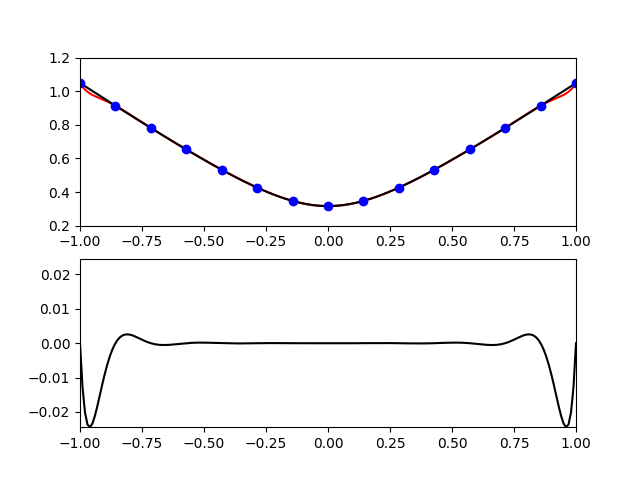
\includegraphics[width=0.80\textwidth]{hw4_figure_1}
		\centering
	\end{figure}
	\begin{figure}[H]
		\caption{First kind Chebyshev points}
		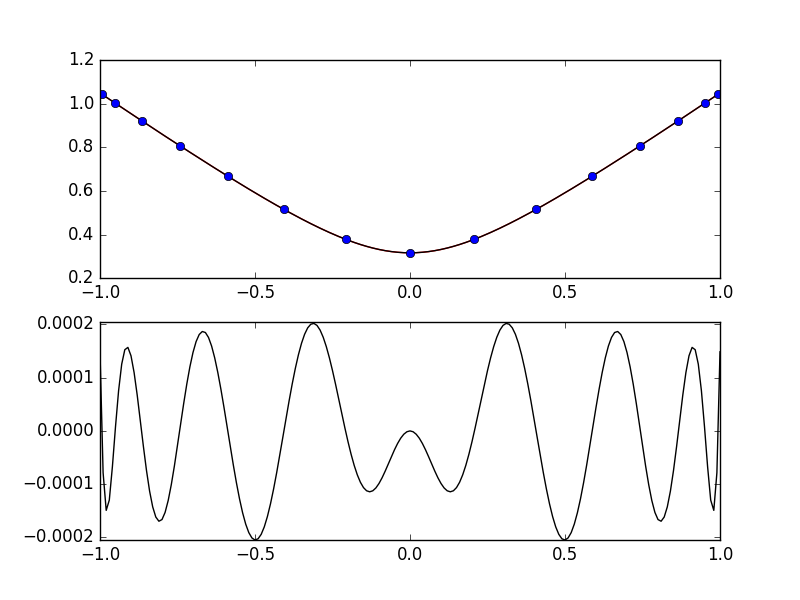
\includegraphics[width=0.80\textwidth]{hw4_figure_2}
		\centering
	\end{figure}
	\begin{figure}[H]
		\caption{Second kind Chebyshev points}
		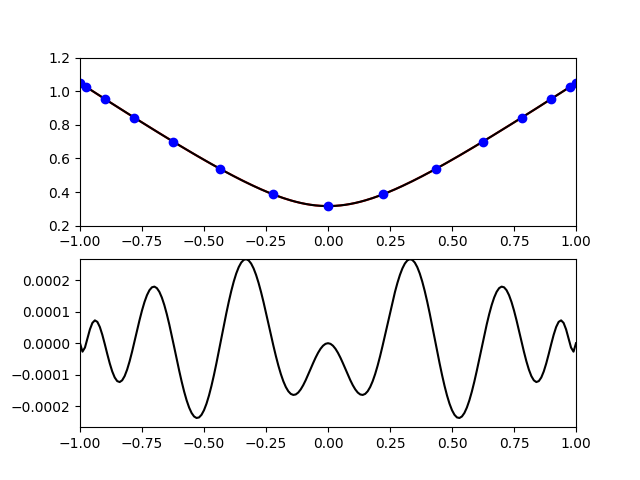
\includegraphics[width=0.80\textwidth]{hw4_figure_3}
		\centering
	\end{figure}
	\begin{figure}[H]
		\caption{Legendre points}
		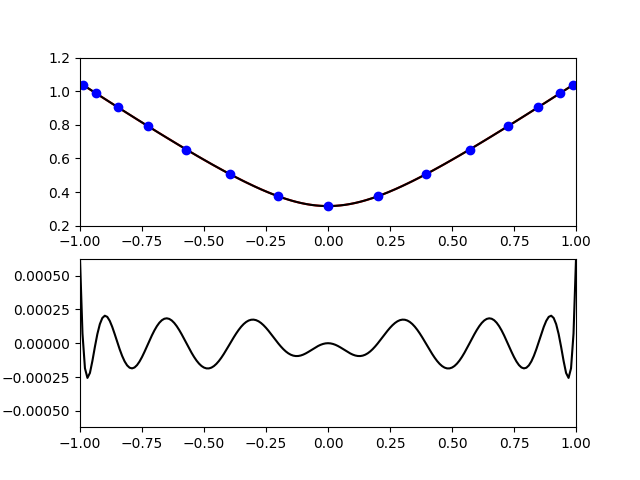
\includegraphics[width=0.80\textwidth]{hw4_figure_4}
		\centering
	\end{figure}

	In each of the four figures the top subplot has the function $f(x) = \sqrt{x^2 + .1}$  in black, along with the interpolating polynomial in red, and the sample points in blue. The bottom subplot has the difference between the function and the interpolating polynomial. Note that the interpolating polynomial is so close to the function in figures 2-3 that it is not visible. \bigbreak
	
	Based off of the 2-norm and the $\infty$-norm any of these pointsets other than the equispaced very closely approximates our function. The Chebyshev points of the first kind minimize both the 2-norm and the $\infty$-norm but not by much. From the graph of the error of the polynomial that interpolates $f$ at the Legendre points, we can see that it is a better estimation for values not near the end points and may be a better predictor than the polynomial interpolating $f$ at the Chebyshev points. \bigbreak
	
%***************************************************************************************************
\problem{4 (c)} Show that for equally spaced points between $[-1,1]$, that 
$$
w_j = \frac{ (\tfrac{n}{2})^n (-1)^{n-j} }{ n! }  {{n}\choose{j}}
$$

	\begin{proof}
		Choose $x_j = -1 + \tfrac{2j}{n}$ for $j = 0, 1, \dots, n$.
		\begin{align*}
			w_j^{-1} & = \prod_{i=0}^{j-1}(x_j - x_i) \prod_{i=j+1}^{n}(x_j - x_i) \\
			& = \prod_{i=0}^{j-1} \frac{2(j-i)}{n} \prod_{i=j+1}^{n} \frac{(-1)2(i-j)}{n} \\
			& = \frac{ 2^{j} (j)!}{ n^{j-1}} \frac{(-1)^{n-j} 2^{n-j} (n-j)!}{ n^{n-j}} \\
			& = \big( \tfrac{2}{n} \big)^{n} (-1)^{n-j} (j)! (n-j)!
		\end{align*}
		Then
		$$
		w_j = w_j \frac{n!}{n!} = \frac{ (\tfrac{n}{2})^n (-1)^{n-j} }{ n! } \frac{n!}{j!(n-j)!} = \frac{ (\tfrac{n}{2})^n (-1)^{n-j} }{ n! }  {{n}\choose{j}}
		$$
	\end{proof}

%***************************************************************************************************
\problem{5 (a)} The only set of specifications you get from SNCF say that the switching path is supposed
to pass through the points $(0, 0), (2, 1)$, and $(4, 2)$. Write down the interpolating polynomial
to this data in both Lagrange form Newton divided difference form (you don’t
need to simplify these). Plot the resulting curve for the train path (using some software
package like Matlab) and include the horizontal lines $y = 0$ and $y = 2$ in your plot.
Also, report the value of the slope of the path at the point $x = 2$. Turn in your work for
computing the polynomial, the plots, and the slope.

	The Lagrange polynomial is expressed as follows:
	$$
	P_2(x) = 0 \frac{ (x-2)(x-4) }{(0-2)(0-4) } + 1 \frac{ (x-0)(x-4) }{(2-0)(2-4) } + 2 \frac{ (x-0)(x-2) }{(4-0)(4-2) } \\
	$$

	For the Newton divided difference form we must first calculate the divided difference table.
	\begin{center}
		\begin{tabular}{|c|c|c|c|}\hline
			$x_i$ & $f(x_i)$ & $f[x_{i-1},x_i]$ & $f[x_{i-2}, x_{i-1}, x_i]$ \\ \hline
			0 &0 & & \\ \hline
			2 &1 & $\tfrac{1}{2}$ & \\ \hline
			4 &2 & $\tfrac{1}{2}$ & 0 \\ \hline
		\end{tabular}
	\end{center}
	
	Then the Newton divided difference form is
	$$
	P_2(x) = 0 + \tfrac{1}{2}(x-0) + 0(x-0)(x-2)
	$$
	
	From the data it is obvious that the interpolating polynomial is just the straight line $y=\tfrac{1}{2}x$ wich has a slope of $\tfrac{1}{2}$. The plot below confirms this.	
	\begin{figure}[H]
		\caption{The interpolating polynomial}
		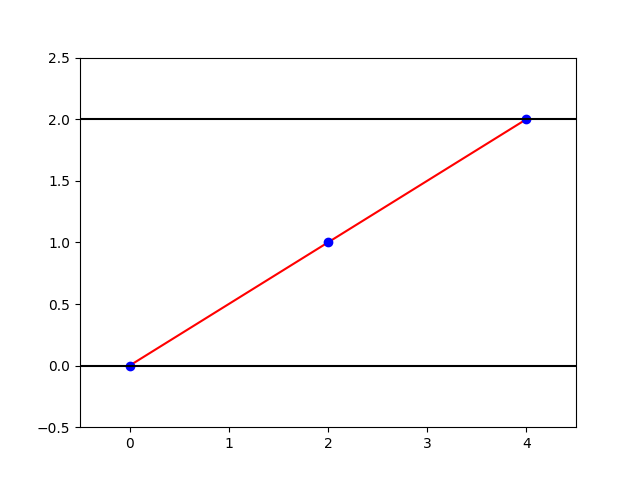
\includegraphics[width=0.75\textwidth]{hw4_figure_5}
		\centering
		\label{fig:p5a}
	\end{figure}
	In figure \ref{fig:p5a}, the interpolating polynomial is in red, the sample points are in blue, and the train tracks are in black.
	
%***************************************************************************************************
\problem{5 (b)} Adding the constraints that $f^\prime(0) = 0 = f^\prime(4)$ we calculate the divided difference

	\begin{center}
		\begin{tabular}{|c|c|c|c|c|c|}\hline
			$x_i$ & $f(x_i)$ & $f[x_{i-1},x_i]$ & $f[x_{x-2}, x_{i-1}, x_i]$ & $f[ x_{i-3}x_{i-2}, x_{i-1}, x_i]$ & $f[ x_{i-4},\dots, x_i]$ \\ \hline
			0 &0 & & & & \\ \hline
			0 &0 & 0 & & & \\ \hline
			2 &1 & $\tfrac{1}{2}$ & $\tfrac{1}{4}$ & & \\ \hline
			4 &2 & $\tfrac{1}{2}$ & 0 & $-\tfrac{1}{16}$ & \\ \hline
			4 &2 & 0 &  $-\tfrac{1}{4}$ & $-\tfrac{1}{16}$ & 0 \\ \hline
		\end{tabular}
	\end{center}

	Then our polynomial becomes
	$$
	P_4(x) = \tfrac{1}{4}(x-0)^2 - \tfrac{1}{16}(x-0)^2(x-2)
	$$
	
	We can simplify this and take the derivative
	\begin{align*}
		P_4(x) & = \tfrac{1}{4}(x-0)^2 - \tfrac{1}{16}(x-0)^2(x-2) \\
		& = \tfrac{1}{4}x^2 - \tfrac{1}{16}x^3 + 2\tfrac{1}{16}x^2 \\
		& = \tfrac{3}{8}x^2 - \tfrac{1}{16}x^3\\
		P_4^\prime(x) = \tfrac{3}{4}x - \tfrac{3}{16}x^2
	\end{align*}
	Then our derivative at $x=2$ is $P_4^\prime(2) = \tfrac{3}{4}$.

	\begin{figure}[H]
		\caption{The interpolating polynomial with zero slope at the end points}
		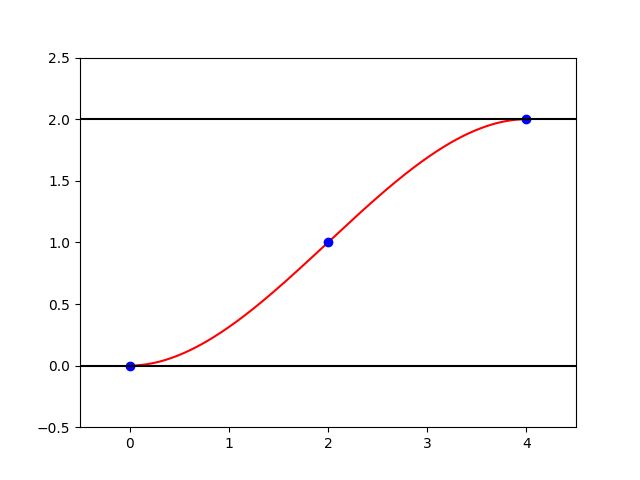
\includegraphics[width=0.75\textwidth]{hw4_figure_6}
		\centering
		\label{fig:p5b}
	\end{figure}
	In figure \ref{fig:p5b}, the interpolating polynomial is in red, the sample points are in blue, and the train tracks are in black. \bigbreak
	
%***************************************************************************************************
\problem{6(c)} Using the same constraints we can also fit two piecewise polynomials that meet at $(2,1)$ and each having slope $1$. Additionally add the condition that the curves have a second derivative of zero at the ends.

	First we construct the divided difference table for the first piece.
	\begin{center}
		\begin{tabular}{|c|c|c|c|c|c|}\hline
			$x_i$ & $f(x_i)$ & $f[x_{i-1},x_i]$ & $f[x_{x-2}, x_{i-1}, x_i]$ & $f[ x_{i-3}x_{i-2}, x_{i-1}, x_i]$ & $f[ x_{i-4},\dots, x_i]$ \\ \hline
			0 & 0 & & & & \\ \hline
			0 & 0 & 0 & & & \\ \hline
			0 & 0 & 0 & 0 & & \\ \hline
			2 & 1 & $\tfrac{1}{2}$ & $\tfrac{1}{4}$ & $\tfrac{1}{8}$ & \\ \hline
			2 & 1 & 1 &  $\tfrac{1}{4}$ & 0 & $-\tfrac{1}{16}$ \\ \hline
		\end{tabular}
	\end{center}
	
	This gives us the equation $P_4(x) = \tfrac{1}{8}(x-0)^3 - \tfrac{1}{16}(x-0)^3(x-2)$ for $0 \leq x \leq 2$. Next we find calculate the divided difference table for the second piece.
	\begin{center}
		\begin{tabular}{|c|c|c|c|c|c|}\hline
			$x_i$ & $f(x_i)$ & $f[x_{i-1},x_i]$ & $f[x_{x-2}, x_{i-1}, x_i]$ & $f[ x_{i-3}x_{i-2}, x_{i-1}, x_i]$ & $f[ x_{i-4},\dots, x_i]$ \\ \hline
			2 & 1 & & & & \\ \hline
			2 & 1 & 1 & & & \\ \hline
			4 & 2 & $\tfrac{1}{2}$ & $-\tfrac{1}{4}$ & & \\ \hline
			4 & 2 & 0 & $-\tfrac{1}{4}$ & 0 & \\ \hline
			4 & 2 & 0 &  0 & $\tfrac{1}{8}$ & $\tfrac{1}{16}$ \\ \hline
		\end{tabular}
	\end{center}
	This gives us the polynomial $Q_4(x) = 1 + 1(x-2) - \tfrac{1}{4}(x-2)^2 + \tfrac{1}{16}(x-2)^2(x-4)^2$ where $2 \leq x \leq 4$. In figure \ref{fig:p5c}, $P_4$ is in red, $Q_4$ is in green, the sample points are in blue, and the train tracks are in black. \bigbreak
	\begin{figure}[H]
		\caption{The interpolating polynomial with zero slope at the end points}
		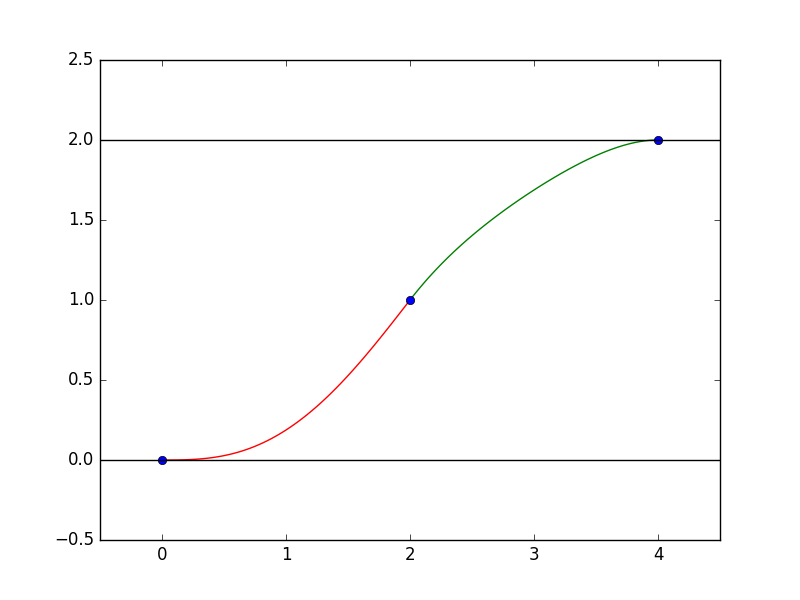
\includegraphics[width=0.75\textwidth]{hw4_figure_7}
		\centering
		\label{fig:p5c}
	\end{figure}
	In figure 

	
	

%***************************************************************************************************
\problem{6(a)} Show that the Chebyshev polynomials $T_n(x)=\cos{(n \arccos{x})}$ satisfy the following properties \\
\emph{(i)} $T_n(1) = 1$ \\
\emph{(ii)} $T_n(-1) = (-1)^n$ \\
\emph{(iii)} $T_j(x)T_k(x) = \tfrac{1}{2}[T_{j+k}(x) + T_{j-k}(x)]$ for $j>k\leq 0$. \\
\emph{(iv)} $\frac{T_{n+1}^\prime(x)}{n+1} - \frac{T_{n-1}^\prime(x)}{n-1} = 2T_n(x)$ for $n=1, 2, ...$ \\

	\begin{proof}
		Clearly $T_n(1) = \cos{(n \arccos{1})} = \cos{(n*0)} = \cos{(0)} = 1$, and thus we have (\emph{i}). \\
		
		In a similar fashion $T_n(-1) = \cos{(n \arccos{-1})} = \cos(n\pi)$ If $n$ is even $T_n(-1) = 1$ and if $n$ is odd then $T_n(-1)=-1$. This is also the case for $(-1)^n$. Thus $T_n(-1) = (-1)^n$ and we have (\emph{ii}). \\
		
		Recall the trig identity $cos(x)cos(y) = \tfrac{1}{2}[cos(x+y) + cos(x-y)]$, which will be useful in proving (\emph{iii}). Then
		\begin{align*}
			T_j(x)T_k(x) & = \cos(j \arccos{x}) \cos(k \arccos{x}) \\
			& = \tfrac{1}{2}[ \cos(j \arccos{x} + k \arccos{x}) +  \cos(j \arccos{x} k - k \arccos{x}) ] \\
			& = \tfrac{1}{2}[ \cos( (j + k) \arccos{x}) + \cos( (j - k) \arccos{x}) ]\\
			& = \tfrac{1}{2}[ T_{j+k}(x) + T_{j-k}(x)]
		\end{align*}
		Thus we have (\emph{iii}). \bigbreak
		
		For (\emph{iv}) it will be useful to recall that $\sin(x+y) - \sin(x-y) = 2 \cos(x) \sin(y)$ and that $\sin(\arccos(x)) = \sqrt{1-x^2}$. Also note that $T_n^\prime = -\sin{(n \arccos{x})} (-n)(1-x^2)^{-\frac{1}{2}}$. Then
		\begin{align*}
			\frac{T_{n+1}^\prime}{n+1} - \frac{T_{n-1}^\prime}{n-1} & = \frac{(n+1) \sin\big((n+1) \arccos(x) \big)}{(n+1)\sqrt{1-x^2}} - \frac{(n-1) \sin\big((n-1) \arccos(x) \big)}{(n-1)\sqrt{1-x^2}} \\
			& = \frac{ \sin\big((n+1) \arccos(x) \big) - \sin\big((n-1) \arccos(x) \big) } { \sqrt{1-x^2} } \\
			& =  \frac{2 \cos(n \arccos(x)) \sin(\arccos(x))}{ \sin(\arccos(x))} \\
			& = 2 T_n(x)
		\end{align*}
		Thus we have (\emph{iv}).		
	\end{proof}

%***************************************************************************************************
\problem{6 (b)} Prove that the Chebyshev polynomials are solutions to the differential equation
	
	\begin{align}\label{p1eq2}
	(1-x^2)y^{\prime\prime}-xy^\prime+n^2y=0
	\end{align}
	
	\begin{proof}
		Note that if $y = T_n(x)$, then
		\begin{align*}
		y^\prime & = -\sin{(n \arccos{x})} \tfrac{d}{dx}(n \arccos{x}) \\
		& = -\sin{(n \arccos{x})} (-n)(1-x^2)^{-\frac{1}{2}} \\
		& = n(1-x^2)^{-\frac{1}{2}}\sin{(n \arccos{x})}  \\
		y^{\prime\prime} &= -\tfrac{n}{2}(1-x^2)^{-\frac{3}{2}}(-2x)\sin{(n \arccos{x})} + n(1-x^2)^{-\frac{1}{2}}\cos{(n \arccos{x})}(-n)(1-x^2)^{-\frac{1}{2}} \\
		&= nx(1-x^2)^{-\frac{3}{2}}\sin{(n \arccos{x})} - n^2(1-x^2)^{-1}\cos{(n\arccos{x})}
		\end{align*}
		Then 
		\begin{align*}
		(1-x^2)y^{\prime\prime} & = (1-x^2) \Big( nx(1-x^2)^{-\frac{3}{2}}\sin{(n \arccos{x})} - n^2(1-x^2)^{-1}\cos{(n\arccos{x})} \Big) \\
		& = nx(1-x^2)^{-\frac{1}{2}}\sin{(n \arccos{x})} - n^2\cos{(n\arccos{x})} \\
		-xy^\prime & = -x n(1-x^2)^{-\frac{1}{2}}\sin{(n \arccos{x})} \\
		n^2y & = n^2\cos{(n \arccos{x})}
		\end{align*}
		Clearly these terms sum to zero and we have our result $(1-x^2)y^{\prime\prime}-xy^\prime+n^2y=0$. Thus $T_n$ are solutions to (\ref{p1eq2}).
		
	\end{proof}

%***************************************************************************************************
\problem{7} Finish the proof we begain in class that the error of the Hermite interpolating polynomial through the points $\{x_i\}_{i=0}^n$ is 
$$
f(x) - p_{2n+1}(x) = [\Phi_{n-1}(x)]^2 \frac{f^{(2n+2)}(\xi)}{(2n+2)!}
$$
for some $\xi \in [x_0, x_n]$, where $\Phi(x) = \prod\limits_{i=0}^n(x-x_i)$.

	\begin{proof}
		In class we constructed the function
		$$
		G(t) = [\Phi_{n+1}(t)]^2 \Big( f(x) - p_{2n+1}(x) \Big) - [\Phi_{n+1}(x)]^2 \Big( f(t) - p_{2n+1}(t) \Big)
		$$
		Note that $\Phi(x_i) = 0$ and $f(x_i) - p_{2n+1}(x_i) = 0$ so $G(x_i)=0$ for $i=0, \dots, n$. Additionally consider the derivative
		\begin{align*}
			\frac{d}{dt}G(t) & = \frac{d}{dt} [\Phi_{n+1}(t)]^2 \Big( f(x) - p_{2n+1}(x) \Big) - [\Phi_{n+1}(x)]^2 \Big( \frac{d}{dt}f(t) - \frac{d}{dt}p_{2n+1}(t) \Big) \\
			& = 2\Phi_{n+1}(t) \frac{d}{dt} [\Phi_{n+1}(t)] \Big( f(x) - p_{2n+1}(x) \Big) - [\Phi_{n+1}(x)]^2 \Big( \frac{d}{dt}f(t) - \frac{d}{dt}p_{2n+1}(t) \Big)
		\end{align*}
		Since $\Phi(x_i) = 0$, and $\frac{d}{dt}f(x_i) - \frac{d}{dt}p_{2n+1}(x_i) = 0$ we know that $G^\prime(x_i) = 0$. Thus $\{x_i\}_{i=0}^n$ are each double roots of $G$. It is also obvious that $G(x) = 0$. Thus $G(x)$ has $n+3$ roots (including multiplicity) over the interval $[x_0,x_n]$. By the generalized Rolle's theorem, there exists $\xi \in [x_0,x_n]$ such that $G^{(2n+2)}(\xi) = 0$. Consider the derivative
		\begin{align*}
			G^{(2n+2)}(t) & = \Big( [\Phi_{n+1}(t)]^2 \Big)^{(2n+2)} \Big( f(x) - p_{2n+1}(x) \Big) \\
			& \text{\ \ \ } - [\Phi_{n+1}(x)]^2 \Big( f^{(2n+2)}(t) - p_{2n+1}^{(2n+2)}(t) \Big)	
		\end{align*}
		Note that $[\Phi_{n+1}(t)]^2$ is a $2n+2$th degree monic polynomial and thus \\
		$\Big( [\Phi_{n+1}(t)]^2 \Big)^{(2n+2)} = (2n+2)!$. Since $p_{2n+1}(x)$ is a $2n+1$st degree polynomial $p_{2n+1}^{(2n+2)}(t) = 0$. Substituting these into our result from Rolle's theorem we have
		$$
		0 = G^{(2n+2)}(\xi) = (2n+2)! \Big( f(x) - p_{2n+1}(x) \Big) - [\Phi_{n+1}(x)]^2 f^{(2n+2)}(\xi)
		$$
		Simple algebra then gets us to the desired result
		$$
		f(x) - p_{2n+1}(x) = [\Phi_{n-1}(x)]^2 \frac{f^{(2n+2)}(\xi)}{(2n+2)!}
		$$
	\end{proof}

%***************************************************************************************************
\problem{8} Suppose that the barycentric weights $w_j , j = 0, 1, . . . , n$ have been computed for some interpolation problem involving the points $\{x_0, x_1, . . . , x_n\}$, so that the $n$th degree interpolating polynomial $p_n(x)$ to some function values $\{f_0, f_1, . . . , f_n\}$ can be constructed according to (2). Describe an algorithm requiring $\mathcal{O}(n)$ operations for computing instead the $(n-1)$ degree for the same points except missing some point $x_k$. Additionally find the value of $p_{n-1}(x_k)$. \bigbreak

	The original weights are given by the formula
	$$
	w_j = \Big( \prod\limits_{\substack{ i=0 \\ i\neq j}}^n (x_j-x_i) \Big)^{-1}
	$$
	the new one is
	$$
	w_j^\prime = \Big( \prod\limits_{\substack{ i=0 \\ i\neq j \\ i\neq k}}^n (x_j-x_i) \Big)^{-1}
	$$
	Thus our new weights can be calculated using the formula $w_j^\prime = w_j(x_j-x_k)$. We have $n+1$ weights originally and we need to find $n$ new weights (there is no $w_k^prime$) so it takes $2n$ operations to find the new weights. The barycentric formula then requires 3 operations to calculate each component of the sum in the denominator and then 1 more multiplication for each component of the sum in the numerator. For $n$ components that would be $4n$ operations. Then there are $2n +1$ more operations to find the sums and do the final division. This is an $\mathcal(O)(n)$ algorithm. \bigbreak
	
	We calculate  $p_{n-1}(x_k)$ as follows
	\begin{align*}
		p_{n-1}(x_k) & = \frac{\sum\limits_{\substack{ j=0 \\ j \neq k}}^n \frac{w_j^\prime}{x_k-x_j}f_j}{\sum\limits_{\substack{ j=0 \\ j \neq k}}^n \frac{w_j^\prime}{x_k-x_j}} \\
		& = \frac{\sum\limits_{\substack{ j=0 \\ j \neq k}}^n \frac{w_j(x_j-x_k)}{x_k-x_j}f_j}{\sum\limits_{\substack{ j=0 \\ j \neq k}}^n \frac{w_j(x_j-x_k)}{x_k-x_j}} \\
		& = \frac{\sum\limits_{\substack{ j=0 \\ j \neq k}}^n -w_jf_j}{\sum\limits_{\substack{ j=0 \\ j \neq k}}^n -w_j} \\
		& = \frac{\sum\limits_{\substack{ j=0 \\ j \neq k}}^n w_jf_j}{\sum\limits_{\substack{ j=0 \\ j \neq k}}^n w_j}
	\end{align*}
	
	

\end{document}
